% 2013 全国卷Ⅱ文科第 9 题：四面体正视图的四个选项；虚线表示隐藏棱。
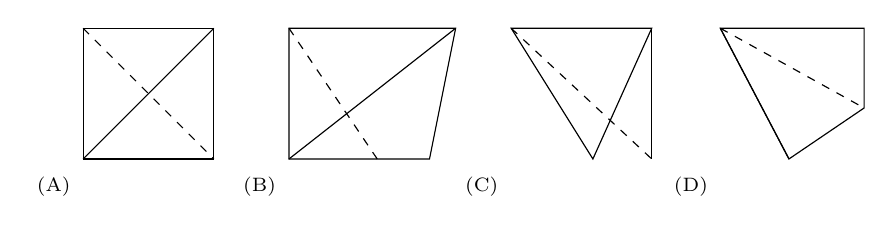
\begin{tikzpicture}[font=\scriptsize, line width=0.42pt, scale=0.83]
  % A
  \begin{scope}
    \node at (-0.45,-0.42) {(A)};
    \draw (0,0)--(2,0)--(2,2)--(0,2)--cycle;
    \draw (0,0)--(2,2);
    \draw[dashed] (0,2)--(2,0);
  \end{scope}
  % B
  \begin{scope}[xshift=3.15cm]
    \node at (-0.45,-0.42) {(B)};
    \draw (0,0)--(2.15,0)--(2.55,2)--(0,2)--cycle;
    \draw (0,0)--(2.55,2);
    \draw[dashed] (0,2)--(1.35,0);
  \end{scope}
  % C
  \begin{scope}[xshift=6.55cm]
    \node at (-0.45,-0.42) {(C)};
    \draw (0,2)--(2.15,2)--(1.25,0)--cycle;
    \draw (2.15,2)--(2.15,0);
    \draw[dashed] (0,2)--(2.15,0);
  \end{scope}
  % D
  \begin{scope}[xshift=9.75cm]
    \node at (-0.45,-0.42) {(D)};
    \draw (0,2)--(2.20,2)--(2.20,0.78)--(1.05,0)--cycle;
    \draw (0,2)--(1.05,0);
    \draw[dashed] (0,2)--(2.20,0.78);
  \end{scope}
\end{tikzpicture}
